\mychapter{Proposed Methodology and System Design}
\vspace{0.5cm}

\subsection{Introduction}

This chapter describes the methodology used to design and implement the proposed \textbf{Digital Admission Script Evaluation and Moderation System (DASEMS)}. It presents the overall system architecture, design approach, software technologies, and interactions among the major components involved in the descriptive admission script evaluation process.

The proposed system digitizes conventional answer script evaluation by integrating role-based access control, secure document management, automated PDF processing, OCR-assisted question segmentation, browser-based evaluation, moderation, and centralized result generation within a single platform. To ensure fairness during evaluation, student identities are concealed using anonymous identifiers, while individual answer regions are extracted from uploaded scripts without altering the original documents.

DASEMS adopts a modular architecture consisting of authentication, administration, document processing, evaluation, and moderation modules. The system is implemented using React with TypeScript for the frontend, Node.js and Express.js for the backend, MongoDB for data management, and Python for PDF processing and OCR. This architecture provides a scalable, maintainable, and efficient solution for descriptive admission script evaluation. The following sections describe the proposed methodology and system design in detail.

\subsection{Research Methodology}

The development of the proposed \textbf{Digital Admission Script Evaluation and Moderation System (DASEMS)} followed a structured software engineering methodology consisting of requirement analysis, system design, implementation, integration, testing, and evaluation. A modular development strategy was adopted because the system contains multiple subsystems, including a web application, backend API, document processing service, and database.

The research methodology adopted in this study is illustrated in Figure~\ref{fig:research_methodology}. The process begins with problem identification and literature review, followed by requirement analysis, system design, implementation, integration, testing, and performance evaluation.

% Keep your existing flowchart here without any modification

The study began with a review of existing admission evaluation systems, OCR techniques, and web-based examination platforms. Based on the identified limitations, the functional and non-functional requirements of DASEMS were analyzed to design the system architecture, database schema, evaluation workflow, and document processing pipeline.

The implementation was carried out incrementally. Core modules such as authentication, user management, admission sessions, and question management were developed first, followed by student registration, PDF upload, and the Python-based document processing service for question detection and answer extraction. An automated assignment module then distributed answers to subject teachers, while the moderation module forwarded inconsistent evaluations to the Head Examiner whenever the predefined threshold was exceeded.

Testing was performed throughout development. Individual modules were verified before integration, and functional testing ensured successful execution of the complete workflow, including authentication, PDF processing, teacher assignment, moderation, and result generation.

The adopted methodology emphasizes modularity, scalability, and maintainability. Since each subsystem performs a specific responsibility, future enhancements such as improved OCR or AI-based handwriting recognition can be incorporated with minimal changes to the overall architecture.

% \begin{figure}[ht]
%     \centering
%     \includegraphics[width=0.75\textwidth]{img/research_methodology.png}
%     \caption{Research methodology adopted for the development of DASEMS.}
%     \label{fig:research_methodology}
% \end{figure}


\begin{figure}[ht]
\centering

\begin{tikzpicture}[
>=Stealth,
process/.style={
draw,
rounded corners=5pt,
thick,
minimum width=7cm,
minimum height=0.8cm,
align=center,
font=\bfseries
},
arrow/.style={
->,
thick
}
]

\node[process,fill=blue!20]    (p1) at (0,0)      {Problem Identification};
\node[process,fill=green!20]   (p2) at (0,-1.5)   {Literature Review};
\node[process,fill=yellow!20]  (p3) at (0,-3.0)   {Requirement Analysis};
\node[process,fill=orange!20]  (p4) at (0,-4.5)   {System Design};
\node[process,fill=cyan!20]    (p5) at (0,-6.0)   {Database Design};
\node[process,fill=purple!20]  (p6) at (0,-7.5)   {Frontend Development};
\node[process,fill=red!20]     (p7) at (0,-9.0)   {Backend Development};
\node[process,fill=teal!20]    (p8) at (0,-10.5)  {PDF Processing Module};
\node[process,fill=lime!20]    (p9) at (0,-12.0)  {Integration};
\node[process,fill=pink!20]    (p10) at (0,-13.5) {Testing and Validation};
\node[process,fill=gray!20]    (p11) at (0,-15.0) {Performance Evaluation};

\draw[arrow] (p1)--(p2);
\draw[arrow] (p2)--(p3);
\draw[arrow] (p3)--(p4);
\draw[arrow] (p4)--(p5);
\draw[arrow] (p5)--(p6);
\draw[arrow] (p6)--(p7);
\draw[arrow] (p7)--(p8);
\draw[arrow] (p8)--(p9);
\draw[arrow] (p9)--(p10);
\draw[arrow] (p10)--(p11);

\end{tikzpicture}

\caption{Research Methodology Workflow}
\label{fig:research_methodology}

\end{figure}



\subsubsection{Development Approach}

DASEMS follows an \textbf{incremental and modular development approach}. The system was divided into independent functional modules that were implemented, tested, and integrated sequentially. This strategy reduced development complexity and simplified debugging.

The implementation was completed in seven phases:

\begin{enumerate}

\item \textbf{Phase 1: Authentication and User Management}

Implemented secure authentication, role-based access control, user registration, password encryption, and JWT-based authorization for Super Administrators, Head Examiners, and Teachers.

\item \textbf{Phase 2: Admission Session and Question Management}

Developed admission session management, subject management, and the digital question bank for configuring examination sessions.

\item \textbf{Phase 3: Student Registration and PDF Upload}

Implemented student registration, anonymous identification, and scanned answer script upload.

\item \textbf{Phase 4: PDF Processing and Answer Segmentation}

Integrated the Python document processing service to detect question boundaries and extract answer regions from uploaded PDFs.

\item \textbf{Phase 5: Teacher Assignment and Evaluation}

Developed automated answer assignment and a browser-based evaluation interface supporting annotations and mark submission.

\item \textbf{Phase 6: Moderation and Result Generation}

Implemented automated moderation by comparing teacher evaluations and forwarding conflicting cases to the Head Examiner before final result generation.

\item \textbf{Phase 7: Reporting and Administrative Dashboard}

Developed dashboards for monitoring evaluation progress, generating reports, and publishing examination results.

\end{enumerate}

The incremental approach enabled continuous testing and reliable integration of each module. The modular architecture also allows future extensions, such as advanced OCR, AI-assisted handwriting recognition, or cloud-based processing, without major modifications to the existing system.

\subsection{Requirement Analysis}

Requirement analysis establishes the functional and operational requirements of the proposed system before implementation. For the proposed \textbf{Digital Admission Script Evaluation and Moderation System (DASEMS)}, requirements were identified by analyzing the conventional admission examination workflow and the responsibilities of administrators, teachers, and head examiners.

The identified requirements are categorized into \textbf{functional} and \textbf{non-functional} requirements. Functional requirements describe the services provided by the system, whereas non-functional requirements define the quality attributes necessary for reliable operation. These requirements form the basis of the proposed system architecture and implementation.

\subsubsection{Functional Requirements}

The major functional requirements of the proposed system are:

\begin{enumerate}

\item \textbf{User Authentication:} Secure login with role-based access for Super Administrator, Head Examiner, and Teacher.

\item \textbf{Examination Management:} Management of admission sessions, departments, subjects, question banks, and student information with anonymous identifiers.

\item \textbf{PDF Processing:} Upload and automatic processing of scanned answer scripts, including question-wise answer segmentation.

\item \textbf{Teacher Assignment and Evaluation:} Automatic assignment of answers to subject-specific teachers and browser-based evaluation with digital annotation and mark submission.

\item \textbf{Moderation:} Automatic detection of significant differences among multiple evaluations and forwarding of disputed answers to the Head Examiner.

\item \textbf{Result Management:} Generation of final results, reports, audit logs, and evaluation statistics.

\end{enumerate}

\subsubsection{Non-Functional Requirements}

The system is designed to satisfy the following quality attributes:

\begin{itemize}

\item \textbf{Security:} JWT-based authentication and role-based authorization.

\item \textbf{Scalability:} Support for large numbers of answer scripts and concurrent users.

\item \textbf{Reliability:} Secure preservation of uploaded scripts and evaluation records.

\item \textbf{Maintainability:} Modular architecture to simplify future enhancements.

\item \textbf{Availability:} Continuous access for evaluators during the examination period.

\item \textbf{Usability and Performance:} Responsive user interface with efficient document processing and evaluation.

\end{itemize}

\subsubsection{User Roles}

The proposed system supports three user roles.

\paragraph{Super Administrator}
Responsible for managing admission sessions, departments, question banks, teachers, students, answer script uploads, evaluation progress, reports, and final result publication.

\paragraph{Teacher}
Evaluates assigned answers through the digital interface, annotates scripts, assigns marks, and submits evaluations without access to student identities or other teachers' assessments.

\paragraph{Head Examiner}
Reviews answers requiring moderation, compares independent evaluations, determines final marks, and approves moderated results before publication.

The separation of responsibilities among these roles improves security, transparency, and efficient management of the admission script evaluation process.


\subsection{Overall System Architecture}

The proposed \textbf{Digital Admission Script Evaluation and Moderation System (DASEMS)} follows a modular multi-layer architecture that separates user interaction, business logic, document processing, and data management into independent components. This layered design improves maintainability, scalability, and reliability while allowing individual modules to communicate through RESTful APIs and shared database services.

The architecture is designed for large-scale university admission examinations, where multiple administrators, teachers, and head examiners perform different tasks simultaneously. Figure~\ref{fig:system_architecture} illustrates the overall architecture of the proposed system.

% \begin{figure}[ht]
%     \centering
%     \includegraphics[width=0.95\textwidth]{img/system_architecture.png}
%     \caption{Overall architecture of the proposed Digital Admission Script Evaluation and Moderation System (DASEMS).}
%     \label{fig:system_architecture}
% \end{figure}

\begin{figure}[H]
\centering

\begin{tikzpicture}[
>=Stealth,
box/.style={
draw,
rounded corners=5pt,
thick,
minimum width=5cm,
minimum height=0.8cm,
align=center,
font=\bfseries
},
smallbox/.style={
draw,
rounded corners=5pt,
thick,
minimum width=2.3cm,
minimum height=0.7cm,
align=center,
font=\small
},
arrow/.style={->,thick}
]

%---------------- Top ----------------%

\node[box,fill=blue!20] (users) at (0,0) {Users};

\node[smallbox,fill=yellow!20] (admin) at (-3,-1.5) {Admin};

\node[smallbox,fill=yellow!20] (teacher) at (0,-1.5) {Teacher};

\node[smallbox,fill=yellow!20] (head) at (3,-1.5) {Head};

\node[box,fill=green!20] (frontend) at (0,-3.5)
{React Frontend};

\node[box,fill=cyan!20] (api) at (0,-5.2)
{REST API Communication};

\node[box,fill=orange!20] (backend) at (0,-7)
{Node.js + Express Backend};

%---------------- Bottom ----------------%

\node[box,fill=purple!20] (mongo) at (-4,-9.3)
{MongoDB Database};

\node[box,fill=red!20] (python) at (4,-9.3)
{Python Processor};

\node[smallbox,fill=purple!10] (m1) at (-4,-11)
{Student Data};

\node[smallbox,fill=purple!10] (m2) at (-4,-12.2)
{Question Bank};

\node[smallbox,fill=purple!10] (m3) at (-4,-13.4)
{Evaluations};

\node[smallbox,fill=purple!10] (m4) at (-4,-14.6)
{Audit Logs};

\node[smallbox,fill=red!10] (p1) at (4,-11)
{OCR Processing};

\node[smallbox,fill=red!10] (p2) at (4,-12.2)
{PDF Segmentation};

\node[smallbox,fill=red!10] (p3) at (4,-13.4)
{Answer Extraction};

\node[smallbox,fill=red!10] (p4) at (4,-14.6)
{Image Cropping};

%---------------- Connections ----------------%

\draw[arrow] (users)--(frontend);

\draw[arrow] (admin)--(frontend);
\draw[arrow] (teacher)--(frontend);
\draw[arrow] (head)--(frontend);

\draw[arrow] (frontend)--(api);
\draw[arrow] (api)--(backend);

\draw[arrow] (backend)--(mongo);
\draw[arrow] (backend)--(python);

\draw[arrow] (mongo)--(m1);
\draw[arrow] (m1)--(m2);
\draw[arrow] (m2)--(m3);
\draw[arrow] (m3)--(m4);

\draw[arrow] (python)--(p1);
\draw[arrow] (p1)--(p2);
\draw[arrow] (p2)--(p3);
\draw[arrow] (p3)--(p4);

\end{tikzpicture}

\caption{Overall System Architecture}
\label{fig:system_architecture}

\end{figure}

The proposed architecture consists of four major layers:

\begin{enumerate}
\item Presentation Layer
\item Application Layer
\item Document Processing Layer
\item Data Layer
\end{enumerate}

Each layer performs specific responsibilities while collaborating to support the complete evaluation workflow.

\subsubsection{Presentation Layer}

It provides a responsive web interface developed using React and TypeScript. Separate dashboards are available for Super Administrators, Teachers, and Head Examiners according to their assigned responsibilities. All communication with the backend occurs through secure RESTful APIs, ensuring that the frontend has no direct access to the database.

\subsubsection{Application Layer}

The application layer, implemented using Node.js and Express.js, contains the core business logic. It manages authentication, admission sessions, question banks, student records, teacher assignment, evaluation, moderation, result generation, and reporting.

\subsubsection{Document Processing Layer}

This is implemented as an independent Python service responsible for analyzing uploaded PDF answer scripts. Separating document processing from the web server improves scalability and prevents computationally intensive OCR operations from affecting application performance.

After a PDF is uploaded, the processor performs embedded text extraction, OCR (when required), question detection, answer segmentation, image cropping, and metadata generation. A hybrid strategy first extracts embedded PDF text and invokes OCR only for scanned documents without a searchable text layer, improving both efficiency and segmentation accuracy.

\subsubsection{Data Layer}

MongoDB serves as the primary database for storing user accounts, admission sessions, question banks, student information, uploaded answer scripts, extracted answer regions, teacher assignments, evaluation records, moderation decisions, audit logs, and final examination results. Its document-oriented architecture provides flexibility. 

\subsubsection{System Workflow}

The workflow begins with administrators configuring admission sessions, uploading question banks, registering students, and submitting scanned answer scripts. The backend forwards uploaded PDFs to the Python processing service, which extracts question-wise answer regions and returns structured metadata.

The backend then automatically assigns extracted answers to subject-specific teachers. Teachers evaluate assigned answers through the web interface using digital annotation tools and submit marks electronically. After evaluation, the moderation module compares submitted marks and forwards answers with significant discrepancies to the Head Examiner. Finally, the system generates examination results, administrative reports, and complete evaluation records for future verification.

The layered architecture separates presentation, business logic, document processing, and data management, resulting in a scalable and maintainable platform. It also provides flexibility for future enhancements, including AI-assisted handwriting recognition, intelligent answer analysis, cloud deployment, and distributed processing.


\subsection{System Modules}

The proposed \textbf{Digital Admission Script Evaluation and Moderation System (DASEMS)} consists of several interconnected functional modules, each responsible for a specific stage of the admission evaluation workflow. The modular design improves maintainability, scalability, testing, and future extensibility by separating authentication, administration, document processing, evaluation, moderation, and reporting into independent components.


\begin{figure}[H]
\centering

\begin{tikzpicture}[
    node distance=0.9cm,
    >=Stealth,
    process/.style={
        rectangle,
        rounded corners=6pt,
        minimum width=7cm,
        minimum height=0.9cm,
        draw=black,
        thick,
        align=center,
        font=\bfseries
    },
    arrow/.style={
        ->,
        thick
    }
]

\node[process,fill=blue!20] (a)
{System Administration};

\node[process,fill=green!20,below=of a] (b)
{Admission Session Management};

\node[process,fill=yellow!25,below=of b] (c)
{Question Bank Management};

\node[process,fill=orange!25,below=of c] (d)
{Student Registration};

\node[process,fill=cyan!25,below=of d] (e)
{PDF Upload \& Processing};

\node[process,fill=purple!20,below=of e] (f)
{Answer Extraction};

\node[process,fill=red!20,below=of f] (g)
{Teacher Assignment};

\node[process,fill=pink!20,below=of g] (h)
{Teacher Evaluation};

\node[process,fill=teal!20,below=of h] (i)
{Moderation};

\node[process,fill=gray!25,below=of i] (j)
{Result Generation};

\draw[arrow] (a) -- (b);
\draw[arrow] (b) -- (c);
\draw[arrow] (c) -- (d);
\draw[arrow] (d) -- (e);
\draw[arrow] (e) -- (f);
\draw[arrow] (f) -- (g);
\draw[arrow] (g) -- (h);
\draw[arrow] (h) -- (i);
\draw[arrow] (i) -- (j);

\end{tikzpicture}

\caption{Overall Admission Examination Workflow}
\label{fig:overall_workflow}

\end{figure}


The workflow begins with admission session configuration and script upload. Uploaded PDFs are processed to extract question-wise answers, which are automatically assigned to subject-specific teachers. After independent evaluation, disputed answers are moderated before final results are generated.

\subsubsection{User Authentication and Authorization Module}

This module provides secure authentication using encrypted passwords and JSON Web Tokens (JWT). Three user roles are supported super administrator, teacher and head examiner.

\subsubsection{Admission Session and Question Bank Module}

This module manages admission sessions, departments, subjects, and digital question banks. Each session maintains examination information, while the question bank stores question numbers, model answers, and marking guidelines. 

\subsubsection{Student Management and Script Upload Module}

This module maintains student information and supports secure PDF upload. Each student is assigned a unique anonymous identifier (\textbf{s\_code}) so that teachers evaluate answers without accessing personal information. Uploaded scripts are validated, stored securely, and forwarded to the document processing module.

\subsubsection{PDF Processing and Answer Extraction Module}

This module automatically analyzes uploaded PDFs to identify question boundaries and extract answer regions. It first attempts embedded text extraction using PDF processing libraries and applies OCR only when necessary. Each extracted answer is saved as an independent image together with metadata such as page number, question number, subject, and coordinates. The original answer script remains unchanged throughout the evaluation process.

\subsubsection{Teacher Assignment Module}

The assignment module automatically distributes extracted answers to subject-specific teachers based on predefined rules. Each answer is assigned to three independent evaluators while balancing workload across available teachers. Assignment records enable administrators to monitor evaluation progress efficiently.

\subsubsection{Teacher Evaluation Module}

Teachers access assigned answers through a browser-based interface displaying the question, model answer, marking guidelines, and extracted answer image. Digital annotation tools allow highlighting, commenting, and marking without modifying the original script. Submitted evaluations are securely stored in the database and cannot be modified without authorization.

\subsubsection{Moderation Module}

After three independent evaluations are completed, the moderation module compares submitted marks. If the variation is within the predefined threshold, the final score is generated automatically. Otherwise, the answer is forwarded to the Head Examiner, who reviews the evaluations and determines the final mark. All moderation activities are permanently recorded for transparency and accountability.

\subsubsection{Result Generation and Reporting Module}

This module consolidates finalized marks, generates examination results, and prepares administrative reports. It also provides statistics on evaluation progress, teacher workload, moderation frequency, and pending assignments. All important system activities are recorded in audit logs, ensuring complete traceability throughout the evaluation process.

\subsection{Database Design}

The proposed \textbf{Digital Admission Script Evaluation and Moderation System (DASEMS)} uses \textbf{MongoDB}, a NoSQL document-oriented database, for storing examination data. Its flexible JSON-like document structure is well suited for managing admission sessions, question banks, student records, answer metadata, evaluations, and audit logs. The database is organized into independent collections linked through unique identifiers, providing scalability, efficient data retrieval, and simplified system maintenance.

Figure~\ref{fig:database_design} illustrates the conceptual database design of the proposed system.

\begin{figure}[H]
    \centering
    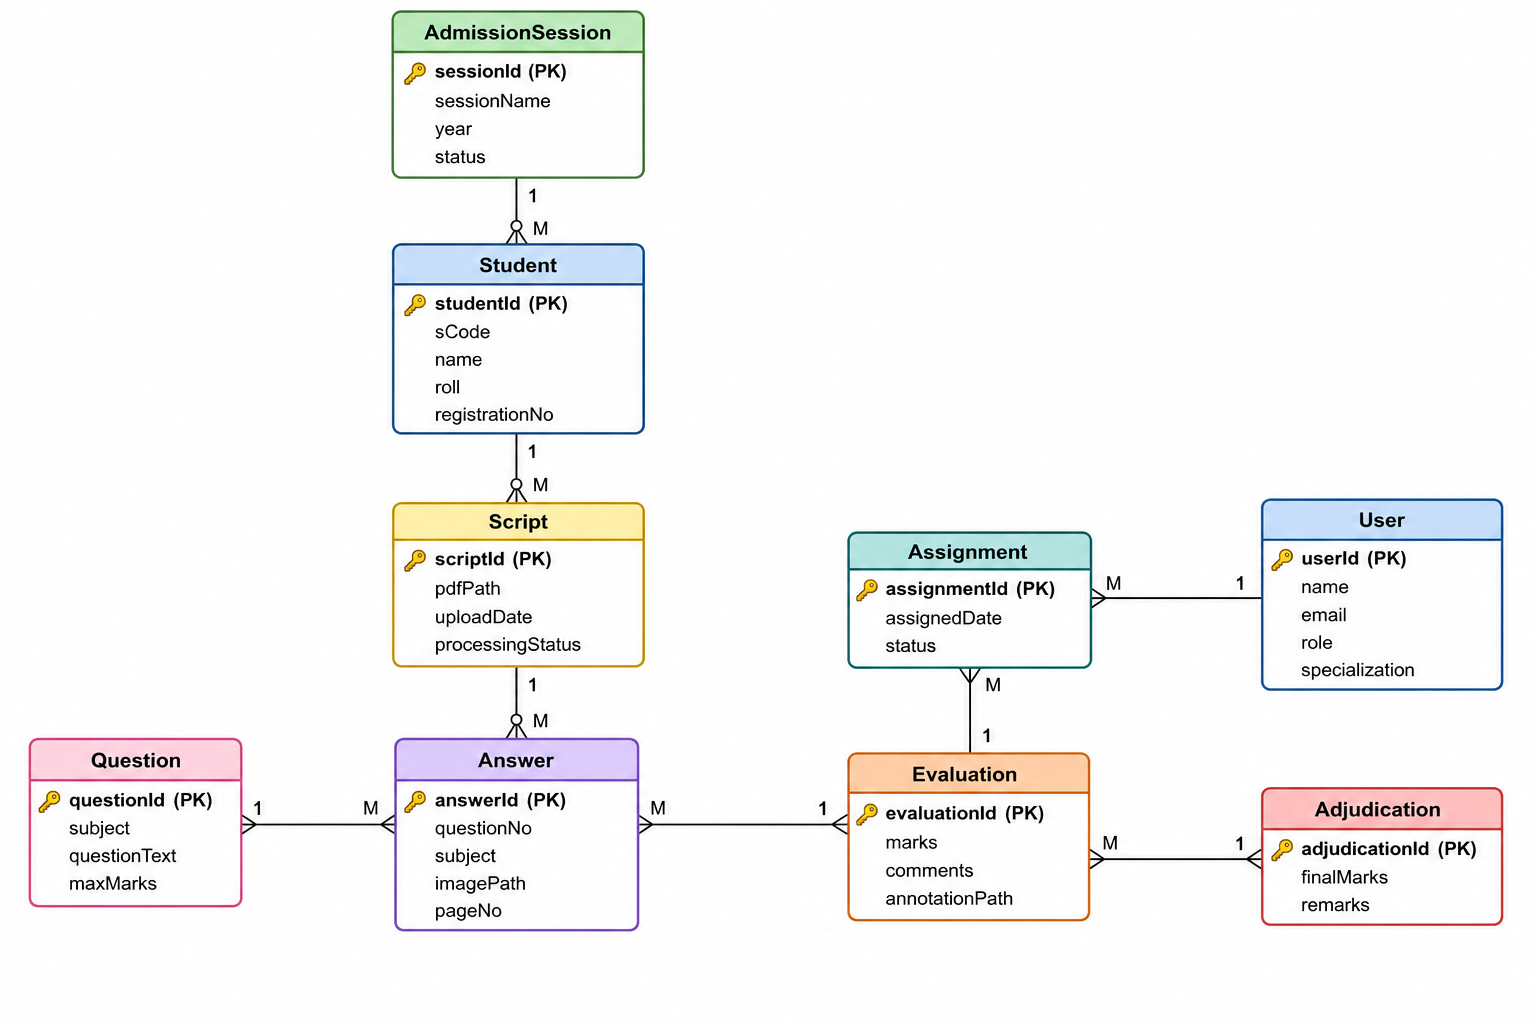
\includegraphics[width=0.90\textwidth]{img/ER_diagram.png}
    \caption{Conceptual database design of the proposed DASEMS.}
    \label{fig:database_design}
\end{figure}




\subsubsection{Database Collections}

The database consists of several major collections that support the admission evaluation workflow.

\begin{itemize}
    \item \textbf{User:} Stores authentication credentials, user profiles, and assigned roles.
    
    \item \textbf{Admission Session:} Maintains examination information including academic year, departments, schedule, and session status.
    
    \item \textbf{Question Bank:} Stores subject-wise questions, model answers, marking rubrics, and maximum marks.
    
    \item \textbf{Student:} Contains student information together with an anonymous identifier (\textbf{s\_code}) used during evaluation.
    
    \item \textbf{Script and Answer:} Store uploaded PDF information and extracted question-wise answer images with their metadata.
    
    \item \textbf{Assignment, Evaluation, and Moderation:} Manage teacher assignments, submitted marks, evaluation records, and moderation decisions.
    
    \item \textbf{Audit Log:} Records important system activities for transparency and future verification.
\end{itemize}

\subsubsection{Entity Relationships}

Each admission session contains multiple students, subjects, and questions. Every student is linked to one uploaded answer script, which is segmented into multiple question-wise answers. Each extracted answer is assigned to three teachers, producing independent evaluation records. When the submitted marks exceed the moderation threshold, the answer is forwarded to the Head Examiner for review. Finalized evaluations are then associated with the corresponding student for result generation, while all activities are recorded in the audit log.

% \subsubsection{Database Design Considerations}

% The database is designed with scalability, performance, and maintainability in mind. Frequently accessed collections are indexed to improve query performance, while uploaded PDFs and answer images are stored separately from the database, with only their metadata being maintained. Evaluation records are treated as immutable to preserve academic integrity, and append-only audit logs ensure complete traceability of all operations.

\subsection{OCR-Based PDF Processing Pipeline}

The OCR-Based PDF Processing Pipeline is the core document processing component of the proposed \textbf{Digital Admission Script Evaluation and Moderation System (DASEMS)}. Its objective is to convert uploaded admission answer scripts into question-wise answer images for digital evaluation. Instead of recognizing handwritten answers, the pipeline identifies question boundaries, extracts answer regions, and generates metadata while preserving the original uploaded PDF.

To improve efficiency, the system adopts a hybrid processing strategy. If the uploaded PDF contains an embedded searchable text layer, question locations are obtained directly using PDF processing libraries. Otherwise, the system automatically applies Optical Character Recognition (OCR) to detect printed question numbers from rendered page images. This approach enables reliable processing of both digital and scanned documents.

% Figure~\ref{fig:ocr_pipeline} illustrates the overall OCR-based processing pipeline.

% \begin{figure}[ht]
%     \centering
%     \includegraphics[width=0.90\textwidth]{img/ocr_pipeline.png}
%     \caption{OCR-Based PDF Processing Pipeline used in DASEMS.}
%     \label{fig:ocr_pipeline}
% \end{figure}

The pipeline consists of several sequential stages, beginning with PDF upload and ending with the generation of structured answer records.

\subsubsection{PDF Upload and Validation}

The pipeline begins when the Super Administrator uploads a PDF answer script. The system validates the file format, integrity, page structure, and admission session before storing the original PDF as a read-only document. This ensures data integrity and prevents invalid files from entering the processing pipeline.

\subsubsection{PDF Rendering}

Validated PDF pages are rendered into high-resolution images using the PyMuPDF library. These images provide the input for OCR and answer extraction when searchable text is unavailable.

\begin{figure}[H]
\centering

\begin{tikzpicture}[
    >=Stealth,
    node distance=0.9cm,
    box/.style={
        rectangle,
        rounded corners=6pt,
        minimum width=5cm,
        minimum height=0.9cm,
        draw=black,
        thick,
        align=center,
        font=\bfseries
    },
    smallbox/.style={
        rectangle,
        rounded corners=5pt,
        minimum width=3.2cm,
        minimum height=0.8cm,
        draw=black,
        thick,
        align=center,
        font=\small\bfseries
    },
    arrow/.style={
        ->,
        thick
    }
]

% Main Flow
\node[box,fill=blue!20] (upload) {PDF Upload};

\node[box,fill=green!20,below=of upload] (validation)
{File Validation};

\node[box,fill=yellow!25,below=of validation] (store)
{Store Original PDF};

\node[box,fill=orange!25,below=of store] (render)
{PDF Rendering};

% Text Layer Detection
\node[box,fill=cyan!25,below=of render] (textlayer)
{Text Layer Detection};

% Branches
\node[smallbox,fill=green!15] (text)
at (-3,-6)
{Question\\Detection};

\node[smallbox,fill=red!15] (ocr)
at (3,-6)
{OCR\\Detection};

% Merge
\node[box,fill=purple!20] (boundary)
at (0,-8)
{Question Boundary Identification};

\node[box,fill=orange!20,below=of boundary]
(crop){Answer Region Cropping};

\node[box,fill=pink!20,below=of crop]
(meta){Metadata Generation};

\node[box,fill=teal!20,below=of meta]
(records){Answer Records Created};

% Connections
\draw[arrow] (render)--(textlayer);

\draw[arrow] (textlayer)--node[left]{\scriptsize Text}(text);

\draw[arrow] (textlayer)--node[right]{\scriptsize No Text}(ocr);

\draw[arrow] (text)--(boundary);

\draw[arrow] (ocr)--(boundary);

\draw[arrow] (boundary)--(crop);

\draw[arrow] (crop)--(meta);

\draw[arrow] (meta)--(records);

\end{tikzpicture}

\caption{PDF Processing and Answer Extraction Workflow}
\label{fig:pdf_processing_workflow}

\end{figure}

\subsubsection{Question Detection}

Question detection is performed using a hybrid two-stage approach. The processor first attempts to extract embedded PDF text and its positional coordinates. If no searchable text exists, OCR is applied to the rendered page images to detect printed question numbers and their locations. This strategy improves both processing speed and robustness.

\subsubsection{Answer Region Extraction}

Using the detected question positions, the system determines the boundary of each answer region, crops it as an independent image, and generates metadata including the anonymous student identifier, subject, question number, page number, coordinates, and image location. These records are stored for teacher assignment and evaluation while the original PDF remains unchanged.

\subsubsection{Advantages of the Proposed Pipeline}

The proposed pipeline preserves the original answer script, automates question-wise answer extraction, and reduces administrative effort. The hybrid strategy avoids unnecessary OCR operations while supporting both searchable and scanned PDFs. The extracted answer images become independent evaluation units that enable automatic teacher assignment, parallel evaluation, and efficient moderation for large-scale admission examinations.

\subsubsection*{Algorithm 3.1: OCR-Based Answer Extraction}

\begin{verbatim}
Input:
    Uploaded PDF document

Output:
    Question-wise extracted answer images

Begin

Validate uploaded PDF

Store original PDF

For each page in the document do

    If searchable text exists then

        Extract text layer
        Detect question positions

    Else

        Render page image
        Perform OCR
        Detect question positions

    End If

    Identify answer boundaries

    Crop answer regions

    Save extracted answer image

    Generate metadata

End For

Store extracted answer records

Return extracted answers

End
\end{verbatim}



\subsection{Teacher Assignment and Moderation Algorithm}

After question-wise answer extraction, the proposed system automatically assigns each answer to qualified teachers for evaluation. The assignment mechanism ensures subject compatibility, balanced workload distribution, and independent evaluation while reducing the administrative effort associated with manual script distribution.

Each extracted answer contains metadata such as subject, question number, anonymous student identifier, and answer image location. Based on the subject, the system retrieves eligible teachers and assigns the answer to three evaluators with the lowest current workload. Teachers can access only their assigned answers and cannot view the evaluations submitted by others, ensuring unbiased assessment.

\subsubsection*{Algorithm 3.2: Teacher Assignment}

\begin{verbatim}
Input : Extracted Answer, Teacher List
Output: Three Assignment Records

Retrieve teachers by subject
Sort by current workload
Assign first three teachers
Store assignment records
Return assignments
\end{verbatim}

\subsubsection{Moderation Process}

To improve evaluation reliability, every answer is independently evaluated by three teachers. After all evaluations are submitted, the system calculates the mark spread:

\begin{equation}
Spread=\max(M_1,M_2,M_3)-\min(M_1,M_2,M_3)
\end{equation}

If

\begin{equation}
Spread \leq T
\end{equation}

the final mark is calculated as

\begin{equation}
FinalMark=\frac{M_1+M_2+M_3}{3}
\end{equation}

Otherwise, the answer is forwarded to the Head Examiner for moderation. The Head Examiner reviews the extracted answer, marking rubric, teacher annotations, comments, and assigned marks before determining the final score. The moderation decision is then stored in the database together with the review information.

\subsubsection*{Algorithm 3.3: Moderation Process}

\begin{verbatim}
Input : Three Teacher Evaluations
Output: Final Evaluation

Calculate mark spread

If spread <= threshold
    FinalMark = Average(M1,M2,M3)
Else
    Send to Head Examiner
    Receive moderated mark
End If

Store final result
\end{verbatim}

\subsection{Security and Authentication}

Security is a key aspect of the proposed \textbf{Digital Admission Script Evaluation and Moderation System (DASEMS)} as it handles confidential admission data and evaluation records.

The system uses encrypted password hashing for user authentication and JSON Web Tokens (JWT) for secure session management. Passwords are never stored in plain text, and only valid tokens are allowed to access protected resources.

Role-Based Access Control (RBAC) restricts system access according to user roles: \textbf{Super Administrator}, \textbf{Teacher}, and \textbf{Head Examiner}. Teachers can evaluate only assigned scripts, while student identities remain hidden through anonymous identifiers to ensure unbiased assessment.

\subsection{Deployment Architecture}

The proposed DASEMS adopts a modular deployment architecture that separates the frontend, backend, document processing service, and database into independent components. This design improves scalability, maintainability, and deployment flexibility.

% Figure~\ref{fig:deployment_architecture} illustrates the deployment architecture of the proposed system.


\begin{figure}[H]
\centering
\begin{tikzpicture}[
    >=Stealth,
    node distance=1.4cm,
    box/.style={
        draw,
        rounded corners,
        thick,
        minimum width=4cm,
        minimum height=1cm,
        align=center,
        font=\bfseries
    },
    smallbox/.style={
        draw,
        rounded corners,
        thick,
        minimum width=3cm,
        minimum height=0.8cm,
        align=center,
        font=\small
    },
    arrow/.style={->,thick}
]

% Main Components
\node[box,fill=blue!20] (frontend) {React Frontend};

\node[box,fill=green!20,below=of frontend] (backend)
{Node.js API Server};

\node[box,fill=orange!20,below left=1.6cm and 2.5cm of backend] (db)
{MongoDB};

\node[box,fill=purple!20,below right=1.6cm and 2.5cm of backend] (python)
{Python Processor};

% Subcomponents
\node[smallbox,fill=orange!10,below=0.9cm of db] (uploads)
{Uploads\\Images};

\node[smallbox,fill=purple!10,below=0.9cm of python] (ocr)
{OCR\\Cropping};

% Connections
\draw[arrow] (frontend) -- (backend);

\draw[arrow] (backend) -- (db);
\draw[arrow] (backend) -- (python);

\draw[arrow] (db) -- (uploads);
\draw[arrow] (python) -- (ocr);

\end{tikzpicture}
\caption{Overall System Component Architecture}
\label{fig:system_component_architecture}
\end{figure}


% \begin{figure}[ht]
%     \centering
%     \includegraphics[width=0.90\textwidth]{img/deployment_architecture.png}
%     \caption{Deployment architecture of the proposed DASEMS.}
%     \label{fig:deployment_architecture}
% \end{figure}



The frontend is developed using React and TypeScript, while the backend is implemented with Node.js and Express.js to manage authentication, evaluation, moderation, and system APIs.

A separate Python service performs PDF processing, OCR, question detection, and answer extraction independently of the web server. MongoDB stores user information, examination data, evaluations, moderation records, and final results. All major services are containerized using Docker to simplify deployment and improve portability. 


